\documentclass[a4paper, 11pt]{article}
\usepackage{amsmath}
\usepackage{amssymb}
\usepackage[T1]{fontenc}
\usepackage[utf8x]{inputenc}
\usepackage{lmodern}
\usepackage{graphicx}
\graphicspath{ {./images/} }
\usepackage[english]{babel} 
\usepackage{natbib}
\usepackage{cite}
\usepackage[parfill]{parskip}
\usepackage{enumerate}
\usepackage{float}%for image positions
\usepackage{hyperref}
\hypersetup{
  colorlinks,
  citecolor=black,
  filecolor=black,
  linkcolor=black,
  urlcolor=black
}
\usepackage{amsthm}
\newtheorem{theorem}{Theorem}[section]
\newtheorem{lemma}[theorem]{Lemma}
\newtheorem{proposition}[theorem]{Proposition}
\newtheorem{axiom}[theorem]{Axiom}
\newtheorem{invariant}[theorem]{Invariant}
\newtheorem{breakpoint}[theorem]{Breakpoint}
\newtheorem{problem}{Problem}
\newtheorem{definition}{Definition} 
\usepackage{algorithm}
\usepackage{algpseudocode}
\usepackage{pifont}
\usepackage{multirow,array}
\usepackage{centernot}
\usepackage{comment} % enables the use of multi-line comments (\ifx \fi) 
\usepackage{lipsum} %This package just generates Lorem Ipsum filler text. 
\usepackage{fullpage} % changes the margin

\begin{document}
\section{Search Heuristics for N-Queens}
\subsection{First-Fail Minimum-Value}
The standard first-fail heuristic is the first-fail minimum-value heuristic, the search tree for it is shown in the figure below. 
\begin{figure}[H]
  \begin{center}
    \scalebox{0.90}{
      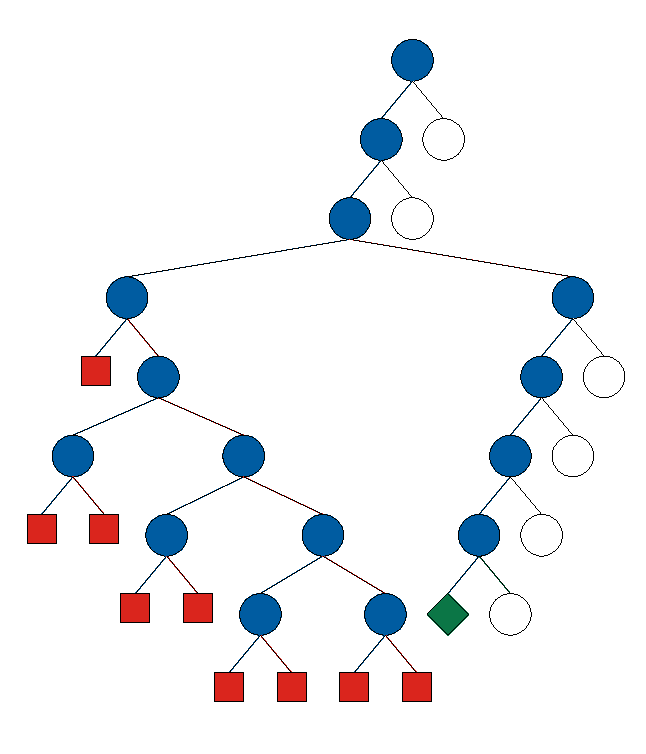
\includegraphics{first_fail_valmin_10.pdf}
    }
    \caption{First-fail Minimum-value for queen problem instance of size 10}
    \label{fig:ffvm10}
  \end{center}
\end{figure}
It visits 25 nodes and 9 failures before finding the first solution.

\subsection{First-Fail Median-domain-value}
\begin{figure}[H]
  \begin{center}
    \scalebox{0.90}{
      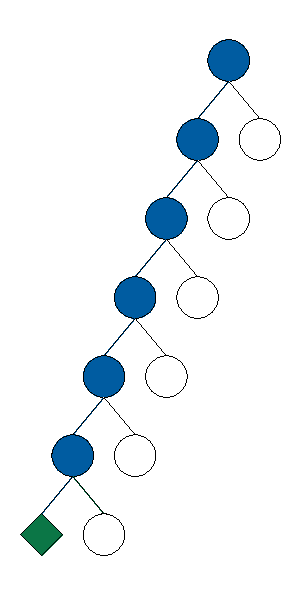
\includegraphics{first_fail_med_10.pdf}
    }
    \caption{First-fail Median-value for queen problem instance of size 10}
    \label{fig:ffmv10}
  \end{center}
\end{figure}
The search visits 7 nodes and 0 failures before finding the first solution.

\subsection{Knight-move heuristic (min-min median-domain-value)}
\begin{figure}[H]
  \begin{center}
    \scalebox{0.90}{
      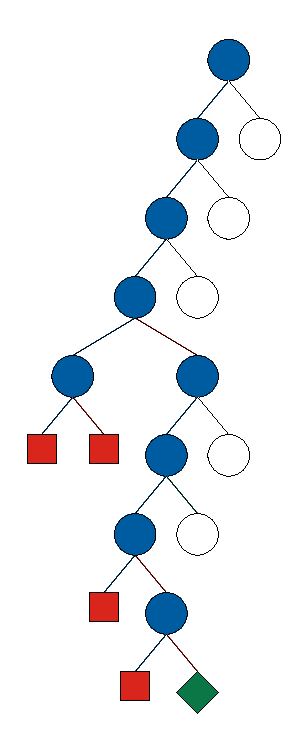
\includegraphics{knight_move_med_10.pdf}
    }
    \caption{Knight-move Median-value for queen problem instance of size 10}
    \label{fig:kmm10}
  \end{center}
\end{figure}
This search visits 14 nodes and 4 failures before finding the first solution.
\subsection{Knight-move heuristic (min-min val-min)}
\begin{figure}[H]
  \begin{center}
    \scalebox{0.60}{
      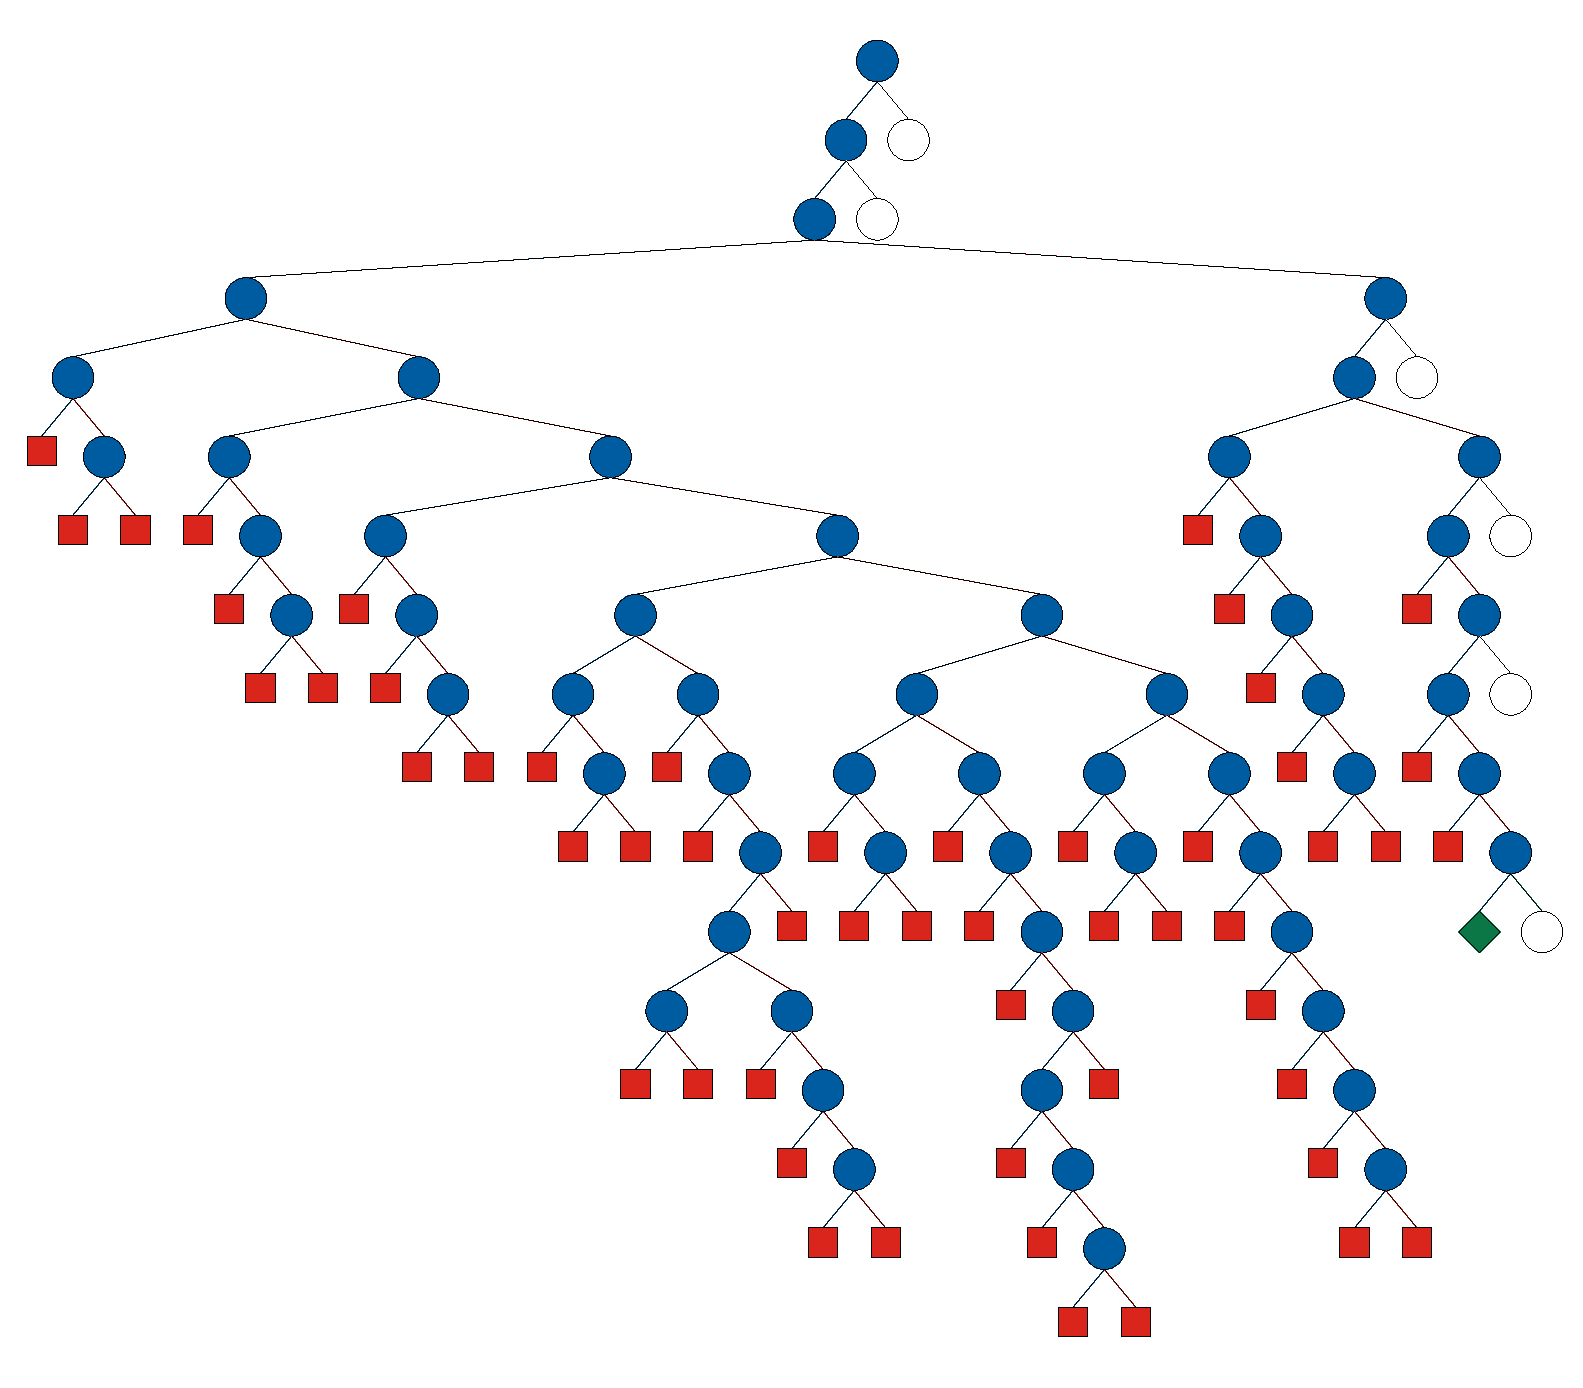
\includegraphics{knight_move_valmin_10.pdf}
    }
    \caption{Knight-move minimum-value for queen problem instance of size 10}
    \label{fig:kmv10}
  \end{center}
\end{figure}
This search visits 113 nodes and 53 failures before finding the first solution.

\section{Conclusion}
Clearly for the problem instance $n = 10$, first-fail median-domain-value was the most effective search heuristic. For $n=10$ we can order the heuristics as follows:

\textit{first-fail median-domain-value (ffmdv)} $\succ$ \textit{knight-move median-domain-value (kmmdv)} $\succ$ \textit{first-fail minimum-value (ffmv)} $\succ$ \textit{knight-move minimum-value (kmmv)}

However what heuristic is best depends a lot on the problem instance. For example as shown in the table below, the first-fail heuristic greatly out-performs the knight-move heuristic for larger n. Also the minimum-value first-fail outperforms the medium-value first-fail for larger n even though medium-value was more efficient for n=10.

\begin{center}
  \begin{tabular}{ | l | l | l | p{7cm} |}
    \hline
    \textbf{Search Heuristic} & \textbf{n} & \textbf{nodes} & \textbf{failures} \\ \hline
    ffmdv & 10 & 25 & 9 \\\hline
    kmmdv & 10 & 14 & 4 \\\hline
    ffmv & 10 & 25 & 9 \\\hline
    kmmv & 10 & 113 & 53 \\\hline
    ffmdv & 100 & 202 & 60 \\\hline
    kmmdv & 100 & ? & ? - No solution in reasonable time \\\hline
    ffmv & 100 & 138 & 22 \\\hline
    kmmv & 100 & ? & ? - No solution in reasonable time \\\hline
    ffmdv & 1000 & 2993 & 998 \\\hline
    kmmdv & 1000 & ? & ? - No solution in reasonable time \\\hline
    ffmv & 1000 & 996 & 2 \\\hline
    kmmv & 1000 & ? & ? - No solution in reasonable time \\\hline    
  \end{tabular}
\end{center}

Why is the heuristic called knight-move heuristic? Because the move that threatens the most other queens and is safe is the knight's move typically.
\end{document}
